\documentclass[10pt]{article}
\usepackage[a4paper, margin = 0.75in, top = 1in]{geometry}
\usepackage[onehalfspacing]{setspace}
\usepackage[hidelinks]{hyperref}
\usepackage[sfdefault]{noto}
\usepackage[T1]{fontenc}
\usepackage{graphicx, fontawesome, calc, enumitem, fancyhdr, kotex}
\setlength{\parindent}{0pt}
\setlength{\tabcolsep}{0pt}
\setlist[itemize, 1]{leftmargin = 0.1in}
\setlist[itemize, 2]{leftmargin = 0.3in}
\NewDocumentCommand \TIME { m o } {%
  \IfValueTF{#2}{#1\newline \enspace to #2}{From #1}%
}
\NewDocumentCommand \HEAD { m } {\raggedleft \textbf{#1} \qquad}
\AtBeginDocument{%
  \pagestyle{fancy}
  \fancypagestyle{stylemain} {%
    \fancyhf{}
    \fancyhead[L]{\textsc{Hyoungjoon ``Paul'' Kim}}
  % \fancyhead[R]{\thepage}
    \fancyfoot[C]{\textsc{curriculum vitae}}
    \renewcommand{\headrulewidth}{0.5pt}
    \renewcommand{\footrulewidth}{0.5pt}
  }
}

\begin{document}
\pagestyle{empty}
\newgeometry{a4paper, margin = 0.5in}

\begin{tabular}{ p{.8\linewidth} p{.2\linewidth} }
  % Name
  {\Large 김형준 \enspace (Hyoungjoon \enspace ``Paul'' \enspace Kim)} \newline
  % One-Liner Description
  % Computer Engineer and Software Developer
  Undergraduate at Electrical \& Computer Engineering,
  Seoul National University \newline
  % Social and Background
  \faFlag{} Republic of Korea \quad
  \faInstitution{} \href{mailto:jsvn7777@snu.ac.kr}{jsvn7777@snu.ac.kr} \quad
  \faEnvelopeO{} \href{mailto:thekpaul000@gmail.com}{thekpaul000@gmail.com}
  \newline
  \faGithub{} \href{https://www.github.com/thekpaul}{thekpaul} \quad
  \faLinkedin{} \href{https://www.linkedin.com/in/thekpaul}{@thekpaul} \quad
% \faHome{} \url{https://thekpaul.dev}
% \newline
  &
  % Profile Picture
  \multicolumn{1}{r}{\raisebox{-\height+11pt}{%
    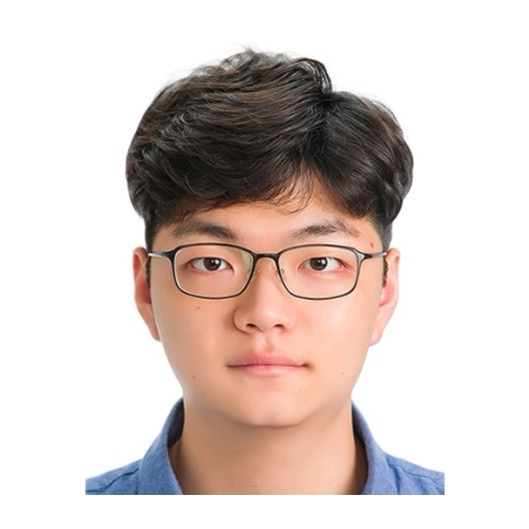
\includegraphics[width = .2\linewidth]{refs/mugshot.png}}}
% \vspace{10pt}
  \\ \hline
\end{tabular}

\begin{center}
  \begin{tabular}{ p{.2\linewidth}  p{.8\linewidth}}
    {\Large Education} & \\[10pt]
    \TIME{Mar. 2018} &
      {\large BS in Electrical \& Computer Engineering,
      Seoul National University} \newline
      Expected to graduate in Summer 2024 \newline
      \textbf{Areas of Interest}: System Programming, Digital Systems Design,
        Deep Learning \newline
      \textbf{Graduation Project}: Optimising the CNN Architecture with
        Hardware Design
    % \\[5pt]
  % \TIME{Mar. 2015}[Feb. 2018] &
  %   {\large Sangmoon High School}
    \\[10pt]
    {\Large Experience} & \\[10pt]
    \TIME{Mar. 2023} &
      {\large FPGA Engineer Intern for \textbf{NeuroRealityVision}} \newline
      Dongtan, Republic of Korea
      \begin{itemize}
        \item Firmware, software development for MIPI-to-Ethernet integration
        \item Bare-metal, standalone FPGA application with interrupt-based
          workflow
        \item Real-time Ethernet packet capture and image rendering
          software development
          \begin{itemize}
            \item Kernel-level optimisations in threading and system calls for
              faster processing speed
            \item Direct modifications to system and network settings
          \end{itemize}
        \item Custom IP development with Verilog-based RTL on Vivado
      \end{itemize}
    \\[-5pt]
    \TIME{Jan. 2023}[Jun. 2023] &
      {\large Student Intern for Dept. of System Semiconductor Engineering}
      \newline
      \textbf{Seoul National University}, Seoul, Republic of Korea
      \begin{itemize}
        \item Worked on CNN Architecture and Hardware Design Optimisation
      \end{itemize}
    \\[-5pt]
    \TIME{Dec. 2019}[Jul. 2021] &
      {\large KATUSA, Human Resources Specialist (42A)} \newline
      \textbf{94\textsuperscript{th} Military Police Battalion},
      Pyeongtaek, Republic of Korea
      \begin{itemize}
        \item Mandatory military service as a KATUSA Agent \newline
          (Korean Augmentation To the United States Army)
      \end{itemize}
    \\[5pt]
  % {\Large Publications} & \\[10pt]
  % \TIME{<++>} &
  %   <++>
  % \\[20pt]
    {\Large Skills} & \\[10pt]
    \HEAD{Engineering} & \vspace{-\baselineskip}
      \begin{itemize}
        \item Experienced in system software engineering for Windows and Linux
        \item Experienced in embedded systems design on multi-purpose SoC FPGAs
        \item Capable of basic RTL hardware design using Verilog
        \item Capable of versatile development with C, C++ and Python
      % \item Capable of maintaining HTML/CSS front-end projects
        \item Proficient in typesetting with \LaTeX{}
      \end{itemize}
      \\[-5pt]
    \HEAD{Languages} & \vspace{-\baselineskip}
      \begin{itemize}
        \item Korean: Native proficiency
        \item English: Fluent, professional working proficiency
      \end{itemize}
    \\
  \end{tabular}
\end{center}

\newpage
\restoregeometry
\pagestyle{stylemain}

\section*{Education}

\subsection*{Bachelor's Degree: ECE, SNU}
\begin{itemize}
  \item Expected to graduate in Summer 2024
  \item \textbf{Graduation Project}: Optimising the CNN Architecture with
    Hardware Design \label{edu:gradproj}
    \begin{itemize}
      \item RTL development with Verilog
      \item Pipelined, streaming CNN architecture concurrently running multiple
        convolution layers
      \item Improved performance in faster speed and less memory usage without
        affecting end results
    \end{itemize}
  \item \textbf{Areas of Interest}: System Programming, Digital Systems Design,
    Deep Learning
  \item[ ] Key Courses Taken:
    \begin{itemize}
      \item Computer Organisation, Digital Systems Design: Basic RTL simulation
        and synthesis on FPGAs
      \item Operating Systems: System calls, tasks, multithreading and
        scheduling on the Linux kernel
      \item Other Computer-related Courses: Introduction to Data Structures,
        Introduction to Algorithms
    \end{itemize}
\end{itemize}

\section*{Experience}

\subsection*{FPGA Engineer Intern: NeuroRealityVision}
\begin{itemize}
  \item Firmware, software development for MIPI-to-Ethernet integration
    \begin{itemize}
      \item Extract MIPI data from normal camera (CIS) and
        \textbf{event camera} (DVS) sensors to FPGA main memory
      \item Experienced in hardware-firmware communication and interrupt
        handling mechanisms
        \begin{itemize}
          \item \textbf{PS} (Processing System): Xilinx Gigabit Ethernet
            Controller (GEM) and ARM Cortex-A53 Processor
          \item \textbf{PL} (Programmable Logic): Xilinx AXI 1G Ethernet
            Subsystem with multiple AXI DMA blocks
        \end{itemize}
      \item Experienced in server-side software development for communication
        with attached FPGA boards \\
        \textit{ex}. Ethernet packet parsing software to receive MIPI data and
          reconstruct image stream
      \item Experienced in system software engineering in multi-threaded
        applications optimised for speed
        \begin{itemize}
          \item Direct interactions with various kernel and OS-specific ABI
            for streamlined performance
          \item Direct modifications to server system to enhance single-core
            and network performance
        \end{itemize}
    \end{itemize}
  \item Custom IP development with Verilog-based RTL on Vivado
    \begin{itemize}
      \item Receive parallel data from attached event camera (DVS) sensor and
        reorganise for AXI4-Stream
      \item Created block designs including RTL blocks to generate IP
      \item Basic experience with generating functioning IPs based on block
        designs in Vivado
    \end{itemize}
  \item Linux Server Management
    \begin{itemize}
      \item Experienced in protocols such as VNC, SSH and RDP for remote work
        and automated services
      \item System administration for wide range of hardware and software
        development toolkits
    \end{itemize}
\end{itemize}

\subsection*{Student Intern: SSAI, SNU}
\begin{itemize}
  \item Research Interest: CNN Architecture and Hardware Design Optimisation
  \item In tandem with \textbf{\hyperref[edu:gradproj]{graduation project}} for
    bachelor's degree from ECE, SNU
\end{itemize}

\subsection*{KATUSA Human Resources Specialist}
\begin{itemize}
  \item Mandatory military service as a KATUSA Agent
    (Korean Augmentation To the United States Army)
  \item Human Resources Specialist (42A) for RSO HHD,
    94th Military Police Battalion at Camp Humphreys
\end{itemize}

% \section*{Skills}

% \subsection*{<++>}

% \subsection*{<++>}

% \subsection*{<++>}

% \subsection*{<++>}

% \subsection*{<++>}

% \subsection*{<++>}

% \subsection*{<++>}

\end{document}
